\documentclass[a4paper,12pt, oneside]{article}
\usepackage{listings}
\usepackage[latin1]{inputenc}
\usepackage{geometry}
\usepackage{pstricks}
\usepackage{graphicx,color}
\usepackage[portuges]{babel}
\usepackage[toc,page]{appendix}
\usepackage{multirow,booktabs}%pacotes para tabelas
\usepackage{amssymb, mathrsfs, amsfonts, amsmath}
\usepackage{amsbsy, hyperref}
\usepackage{latexsym}
\usepackage{booktabs}
\usepackage{yfonts}
\usepackage{tikz}
\usepackage{eurosym} %pacote para o simbolo do euro
\usepackage[titles]{tocloft}
\usepackage{newfloat}%%pacote para criar nova lista
\usepackage[labelfont=rm,format=plain,indention=0cm,singlelinecheck=off,justification=raggedright,skip=2pt]{caption}
\usepackage{chngcntr} %pacote para solucionar a falta de \subsubsubsection
\usepackage{natbib} %pacote para o estilo bibliografico utilizado. \citet, \citep e \citeyearpar
 	% With natbib v5.3, a full list of authors may also follow the year.
	 % In natbib.sty, it is possible to define the type of enclosures that is
	 % really wanted (brackets or parentheses), but in either case, there must
	 % be parentheses in the label.
	 % The \cite command functions as follows:
	 %   \citet{key} ==>>                Jones et al. (1990)
	 %   \citet*{key} ==>>               Jones, Baker, and Smith (1990)
 	%   \citep{key} ==>>                (Jones et al., 1990)
	 %   \citep*{key} ==>>               (Jones, Baker, and Smith, 1990)
	 %   \citep[chap. 2]{key} ==>>       (Jones et al., 1990, chap. 2)
	 %   \citep[e.g.][]{key} ==>>        (e.g. Jones et al., 1990)
	 %   \citep[e.g.][p. 32]{key} ==>>   (e.g. Jones et al., 1990, p. 32)
	 %   \citeauthor{key} ==>>           Jones et al.
		 %   \citeauthor*{key} ==>>          Jones, Baker, and Smith
 	%   \citeyear{key} ==>>             1990	
	
\usepackage{parskip} %pacote para controle de paragrafos
\usepackage{setspace} %pacote para espaçamento entre linhas 
				      %comandos:
						% \singlespacing  -> Para um espaçamento simples
						% \onehalfspacing  -> Para um espaçamento de 1,5
						% \doublespacing  -> Para um espaçamento duplo


 \geometry{
a4paper,total={210mm,297mm},
 left=30mm,right=20mm,
 top=30mm,bottom=20mm,
 } %Dimensoes da pagina

\setcounter{secnumdepth}{6}
\renewcommand\theparagraph{\Alph{paragraph}}

\makeatletter %Solucao para \subsubsubsection
\renewcommand\paragraph{\@startsection{paragraph}{4}{\z@}%
                                     {-3.25ex\@plus -1ex \@minus -.2ex}%
                                     {0.0001pt \@plus .2ex}%
                                     {\normalfont\normalsize}}
\renewcommand\subparagraph{\@startsection{subparagraph}{5}{\z@}%
                                     {-3.25ex\@plus -1ex \@minus -.2ex}%
                                     {0.0001pt \@plus .2ex}%
                                     {\normalfont\normalsize}}
\counterwithin{paragraph}{subsubsection}
\counterwithin{subparagraph}{paragraph}

\counterwithin*{paragraph}{section} 					
\setcounter{tocdepth}{5}% Aumenta o número de níveis do sumário												
\makeatother %Solucao para \subsubsubsection

\setlength{\parindent}{2cm} 
%espaço dos paragrafos. Este comando nao tem efeito no primeiro paragrafo de uma secao.
						
\setlength\parskip{0cm} %ESPACAMENTO ENTRE OS PARAGRAFOS

\setcounter{page}{0} %iniciar a paginacao

\makeatletter %refazendo o formato do cabecalho de uma secao
\renewcommand\@seccntformat[1]{\normalsize{\csname the#1\endcsname}
\hspace{0.1em}} %distancia entre o numero e o titulo da secao
\makeatother

\makeatletter %refazendo o formato do sumario
\renewcommand\l@section            {\bf \@dottedtocline{1}{0em}{4em}}
\renewcommand\l@subsection      {\bf \@dottedtocline{2}{0em}{4em}}
\renewcommand\l@subsubsection{\bf \@dottedtocline{3}{0em}{4em}}
\renewcommand\l@paragraph{\rm \@dottedtocline{4}{0em}{4.5em}}
\renewcommand\l@subparagraph{\rm \@dottedtocline{5}{0em}{4.5em}}


\AtBeginDocument{%refazendo o formato do nome do sumario
\renewcommand\contentsname{\center \normalsize{SUM\'ARIO}}}

\AtBeginDocument{%Refazendo lista de tabelas
\renewcommand\listtablename{\center \normalsize{LISTA DE TABELAS}}
}
\setlength{\cfttabindent}{0em}
\renewcommand{\cfttabpresnum}{Tabela }
\renewcommand{\cfttabaftersnum}{ -- }
\setlength{\cfttabnumwidth}{4.6em}


%Criando lista de graficos
\newlistof{grafico}{graf}{\center \normalsize{\bf LISTA DE GR\'AFICOS}}
\DeclareFloatingEnvironment[name={Gr\'afico},fileext=graf]{grafico}

\setlength{\cftgraficoindent}{0em}
\renewcommand{\cftgraficopresnum}{Gr\'afico }
\renewcommand{\cftgraficoaftersnum}{ -- }
\setlength{\cftgraficonumwidth}{4.8em}


\AtBeginDocument{%Refazendo lista de figuras
\renewcommand\listfigurename{\center \normalsize{LISTA DE FIGURAS}}
}
\setlength{\cftfigindent}{0em}
\renewcommand{\cftfigpresnum}{Figura }
\renewcommand{\cftfigaftersnum}{ -- }
\setlength{\cftfignumwidth}{4.6em}

\geometry{verbose,a4paper,tmargin=30mm,bmargin=20mm,lmargin=30mm,rmargin=20mm}
% Dimensoes da pagina utilizando o pacote geometry

\newtheorem{Cor}{Corol\'ario}[section]
\newtheorem{Prop}{Proposi\c c\~ao}[section]
\newtheorem{Def}{Defini\c c\~ao}[section]
\newtheorem{Teo}{Teorema}[section]
\newtheorem{Lema}{Lema}[section]

%modelo para citação direta com mais de 3 linhas: Inserir no template principal: joao.tex

\newenvironment{quoting}%%% comando para citacao direta com mais de 3 linhas
  {%
   \small\singlespacing
   \begin{list}{}{%
       \setlength{\listparindent}{0cm}%
       \setlength{\itemindent}{\listparindent}%
       \setlength{\rightmargin}{0cm}%
       \setlength{\leftmargin}{4cm}%
       \setlength{\parsep}{0pt}}%
    \item\relax}%
  {\end{list}}


%%%%%%%%%%%%%%%%%%%%%%%%%%%%%%%%%%%%%%%%%%%%%%%%%%%%%%%%%%
%%%%%%%%%%%%%%%%%%%%%%%%%%%%%%%%%%%%%%%%%%%%%%%%%%%%%%%%%%
%%%%%%%%%%%%%%  INICIANDO O DOCUMENTO  %%%%%%%%%%%%%%%%%%%%%%%%%%%%%

\begin{document}					

%%%%%%%%%% ---------------------------------------------%%%%%%%%%%%%%%%
%%%%%%%%%% Informacoes de dados para CAPA  %%%%%%%%%%%%%%%
%%%%%%%%%% ---------------------------------------------%%%%%%%%%%%%%%%

\thispagestyle{empty}

\begin{figure}
\centering

\includegraphics[scale=0.2]{BrasaoUFC.jpg}
\end{figure}

% ATENCAO!!!!!!!!!!!!!!!!!!!!!!!!!!!!!!!!!!!!!
% O arquivo da figura BrasaoUFC.jpg deve estar no mesmo diretorio deste arquivo.

\textcolor[rgb]{1.00,1.00,1.00}{a}

\vspace{-1,2cm}

\centerline{\bf UNIVERSIDADE FEDERAL DO CEAR\'A}

 \centerline{\bf CENTRO DE TECNOLOGIA}

 \centerline{\bf DEPARTAMENTO DE ENGENHARIA DE TELEINFORM\'ATICA} 

\centerline{\bf PROGRAMA DE P\'OS-GRADUA\c C\~AO EM ENGENHARIA DE TELEINFORM\'ATICA}

\vspace{4,25cm}

\centerline{\bf DIEGO PERDIG\~AO SOUSA}

\vspace{4,25cm}

\centerline{\bf INTELIG\^ENCIA COMPUTACIONAL APLICADA}
\centerline{\bf TRABALHO COMPUTACIONAL I}

\vspace{4,25cm}

\begin{center}
{\bf OTIMIZA\c C\~AO USANDO ALGORITMOS DE COMPUTA\c C\~AO EVOLUCION\'ARIA (GA E DE) E INTELIG\^ENCIA DE ENXAME (PSO)}
\end{center}

\vspace{\stretch{1}}
%cidade e data aparecem nas duas ultimas linhas da pagina.
\begin{center}
{\bf FORTALEZA \\  \vspace{0,2 cm} 2017}
\end{center}

\pagebreak  %quebra de pagina






% --------------------------------------------------------------------------
% Informacoes de dados para FOLHA DE DEDICATORIA
% --------------------------------------------------------------------------




%%%%%%%%%% ---------------------------%%%%%%%%%%%%%%%%%%%%%%%
%%%%%%%%%%  LISTA DE FIGURAS %%%%%%%%%%%%%%%%%%%%%%%
%%%%%%%%%% ---------------------------%%%%%%%%%%%%%%%%%%%%%%%

\thispagestyle{empty}

\vspace{0,75cm}

\listoffigures %comando para criar uma lista de figuras

\pagebreak  %quebra de pagina

%%%%%%%%%% -----------------------------%%%%%%%%%%%%%%%%%%%%%%%
%%%%%%%%%%  LISTA DE GRAFICOS %%%%%%%%%%%%%%%%%%%%%%%
%%%%%%%%%% -----------------------------%%%%%%%%%%%%%%%%%%%%%%%

\thispagestyle{empty}

\vspace{0,75cm}

\listofgrafico

\pagebreak  %quebra de pagina

%%%%%%%%%% ---------------------------%%%%%%%%%%%%%%%%%%%%%%%
%%%%%%%%%%  LISTA DE TABELAS %%%%%%%%%%%%%%%%%%%%%%%
%%%%%%%%%% ---------------------------%%%%%%%%%%%%%%%%%%%%%%%

\thispagestyle{empty}

\vspace{0,75cm}

\listoftables %comando para criar uma lista de tabelas

\pagebreak  %quebra de pagina

%%%%%%%%%% -------------------------------------------------%%%%%%%%%%%%%%%%
%%%%%%%%%%  LISTA DE ABREVIATURAS E SIGLAS %%%%%%%%%%%%%%%%
%%%%%%%%%% --------------------------------------------------%%%%%%%%%%%%%%%%


%%%%%%%%%% ---------------%%%%%%%%%%%%%%%%%%%%%%%
%%%%%%%%%%  SUMARIO %%%%%%%%%%%%%%%%%%%%%%%
%%%%%%%%%% ---------------%%%%%%%%%%%%%%%%%%%%%%%

\thispagestyle{empty}

\tableofcontents %comando para criar uma lista de referencias

\pagebreak  %quebra de pagina

%%%%%%%%%% ---------------------%%%%%%%%%%%%%%%%%%%%%%%
%%%%%%%%%%  INTRODUCAO %%%%%%%%%%%%%%%%%%%%%%%
%%%%%%%%%% ---------------------%%%%%%%%%%%%%%%%%%%%%%%

%\thispagestyle{empty}

\pagestyle{myheadings}

\onehalfspacing

\section{\normalsize{QUEST\~AO 01}}

\vspace{0,2cm}


\hspace{2cm} Considere a fun\c c\~ao de Rastringin para 2 vari\'aveis:
\begin{equation}
f(x_{1},x_{2})=20+x_{1}^{2}+x_{2}^{2}-10(\cos(2\pi x_{1})+\cos(2\pi x_{2}))
\end{equation}
em que $x_{i}\in[-5,12;+5,12]$, $i=1,2$. Esta fun\c c\~ao possui um m\'inimo global em $(x_{1},x_{2})=(0,0)$ para o qual $f(x_{1},x_{2})=0$. Pede-se:

\subsection{\normalsize{Item $i$}}
%\hspace{2cm} 

\textbf{Enunciado}: Fazer o gr\'afico da fun\c c\~ao $f(x_{1},x_{2})$ para todo o dom\'inio de $(x_{1},x_{2})$. 

\vspace{0,2cm} 
%\lstinputlisting[language=Matlab]{trabalho_01.m}
Para a solu��o do problema, gerou-se uma discretiza��o de 0,01 de  $x_{i}$ para calcular $f(x_{1},x_{2})$ para todo o dom\'inio de $(x_{1},x_{2})$. Com este valor de discretiza��o, o valor de m�nimo global, $f(0,0)$, � calculado. Foram calculados 1.025 pontos de $f(x_{1},x_{2})$.

O gr�fico da fun\c c\~ao $f(x_{1},x_{2})$ para todo o dom\'inio de $(x_{1},x_{2})$ � apresentado na Figura \ref{surf}, 
\begin{figure}[!h]
	\centering
	\captionsetup{width=12.3cm,skip=0pt,labelsep=endash}
	\caption{Gr\'afico da fun\c c\~ao $f(x_{1},x_{2})$ \label{surf}}
	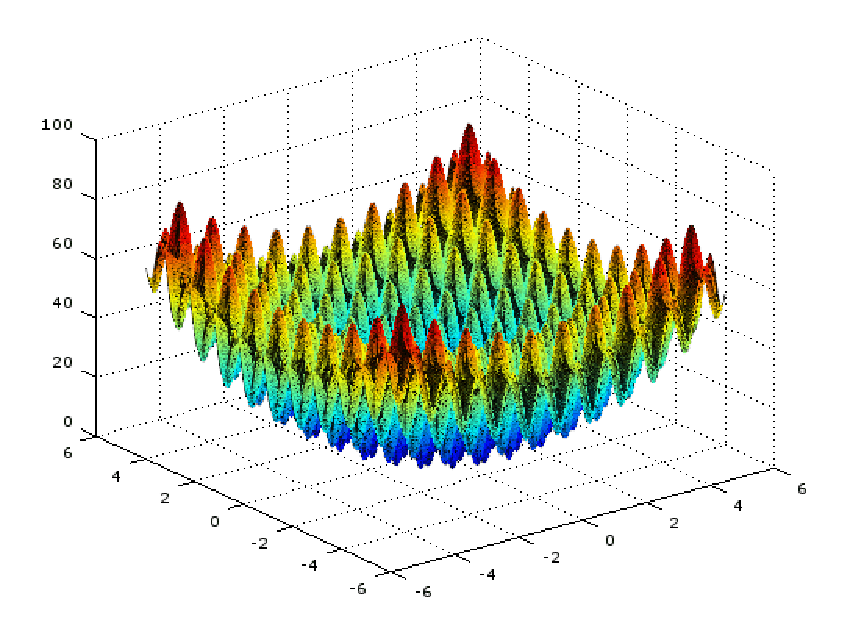
\includegraphics[scale=1.06]{surf}
	%\captionsetup{font=small,position=below,skip=-1pt}
\end{figure}
%\lstinputlisting[firstnumber={183}]{Section_2.m}
%\lstinputlisting{trabalho_01.m}

\subsection{\normalsize{Item $ii$}}
%\hspace{2cm} 

\textbf{Enunciado}: Fazer o gr\'afico das curvas de contorno para esta fun\c c\~ao. 

\vspace{0,2cm} 

O gr�fico das curvas de contorno de $f(x_{1},x_{2})$ � apresentado na Figura \ref{contour}. 
\begin{figure}[!h]
	\centering
	\captionsetup{width=12.3cm,skip=0pt,labelsep=endash}
	\caption{Curvas de contorno de $f(x_{1},x_{2})$ \label{contour}}
	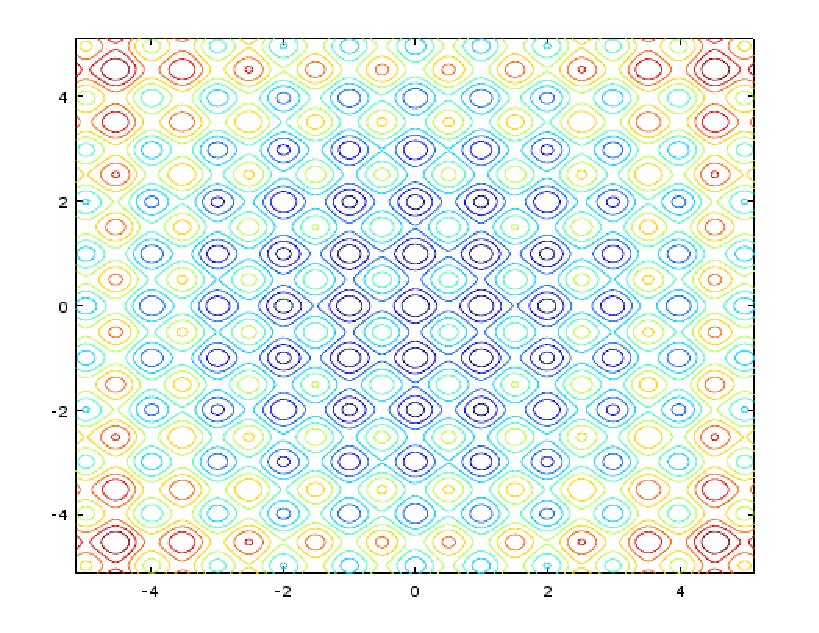
\includegraphics[scale=1.06]{contour}
	%\captionsetup{font=small,position=below,skip=-1pt}
\end{figure} 

As Figuras \ref*{surf} e \ref{contour} foram geradas a partir do c�digo elaborado no Octave mostrado abaixo:

\lstinputlisting[language=Octave, frame=single,numbers=left]{trabalho_01.m}


\subsection{\normalsize{Item $iii$}}
%\hspace{2cm} 

\textbf{Enunciado}: Encontrar o m\'inimo global usando GA usando codifica\c c\~ao real. Mostrar gr\'aficos da fun\c c\~ao de aptid\~ao do melhor indiv\'iduo e da aptid\~ao m\'edia da popula\c c\~ao a cada gera\c c\~ao. Especificar valores adequados dos par\^ametros tamanho da popula\c c\~ao ($N$) e probabilidades de
recombina\c c\~ao ($p_{c}$) e de muta\c c\~ao ($p_{m}$). 

\vspace{0,2cm} 

Para.

\subsection{\normalsize{Item $iv$}}
%\hspace{2cm} 

\textbf{Enunciado}: Avaliar empiricamente o efeito de uma escolha inadequada dos par\^ametros $(N, p_{c}$ e $p_{m})$ no desempenho do AG. Sugest\~ao: Fixar dois dos par\^ametros e verificar como o desempenho do AG \'e afetado pela varia\c c\~ao do terceiro par\^ametro. 

\vspace{0,2cm} 

Para.

\subsection{\normalsize{Item $v$}}
%\hspace{2cm} 

\textbf{Enunciado}: Repetir o experimento usando as metaheur\'isticas evolu\c c\~ao diferencial (DE) e otimiza\c c\~ao
por enxame de part\'iculas (PSO). Compare os resultados obtidos em termos de velocidade de converg\^encia para o \'otimo global, tempo de simula\c c\~ao e insensibilidade a varia\c c\~ao de par\^ametros. 

\vspace{0,2cm} 

Para.

\pagebreak  %quebra de pagina

%%%%%%%%%% -------------------------%%%%%%%%%%%%%%%%%%%%%%%
%%%%%%%%%%  SECAO PRIMARIA %%%%%%%%%%%%%%%%%%%%%%%
%%%%%%%%%% -------------------------%%%%%%%%%%%%%%%%%%%%%%%

\pagestyle{myheadings}

\onehalfspacing

\section{\normalsize{QUEST\~AO 02}}

\vspace{0,2cm}

\hspace{2cm} Considere o problema de ajuste de curvas para os dados do aerogerador disponibilizado no SIGAA. De posse de um conjunto de $N$ pares entrada-sa\'ida ${(v(l),p(l)}_{l=1}^{N}$, assuma
que a curva de regress\~ao \'e um polin\^omio de ordem $k (k\geq 0)$, ou seja
\begin{equation}
p(v)=a_{0}+a_{1}v+a_{2}v^{2}+\cdots+a_{k}v^k,
\end{equation}
em que $v$ \'e a velocidade do vento (m/s) e $p$ \'e a pot\^encia gerada (kW) predita pelo modelo polinomial. Use as metaheur\'isticas DE e PSO para estimar valores para os par\^ametros $a_{j}$, $j =
0,\ldots,k$. Compare o resultado obtido com aquele gerado por fun\c c\~oes prontos do Matlab/Octave (e.g. fun\c c\~ao \textbf{polyfit}) ou do software \textbf{R}.

Dicas: 
\begin{enumerate}
	\item Represente o $i$-\'esimo indiv\'iduo (cromossomo ou part\'icula) do algoritmo como o seguinte
	vetor:
	\begin{equation}
	x_{i}=[a_{0}^{i a_{1}^{i}} \cdots a_{k}^{i}]^{\top} .
	\end{equation}
	
	\item Use como fun\c c\~ao-objetivo a ser minimizada a soma dos erros quadr\'aticos (SEQ):
	\begin{equation}
	f(x_{i})=\sum_{l=1}^{N}e_{i}^{2}(l),
	\end{equation}
	em que $e_{i}(l)=p(l)-$\^p$_{i}(l)$ \'e o erro entre o $l$-\'esimo valor medido de pot\^encia e o valor predito pelo modelo de regress\~ao associado ao $i$-\'esimo indiv\'iduo da popula\c c\~ao. O n\'umero total de pontos no banco de dados \'e $N$.
	
	\item O valor predito pelo modelo de regress\~ao associado ao $i$-\'esimo indiv\'iduo da popula\c c\~ao \'e dado por
	\begin{equation}
	p(l)=a_{0}^{(i)}+a_{1}^{(i)}v(l)+a_{2}^{(i)}v^{2}(l)+\cdots+a_{k}^{(i)}v^{k}(l),
	\end{equation}

\end{enumerate}
%%%%%%%%%% -------------------------------%%%%%%%%%%%%%%%%%%%%%%%
%%%%%%%%%%  SECAO SECUNDARIA %%%%%%%%%%%%%%%%%%%%%%%
%%%%%%%%%% -------------------------------%%%%%%%%%%%%%%%%%%%%%%%

\subsection{\normalsize{T\'itulo da se\c c\~ao secund\'aria}}

\vspace{0,2cm}

\hspace{2cm} Para Siss (\citeyear{Siss}) as pol\'iticas de a\c{c}\~ao afirmativas constituem pol\'iticas p\'ublicas, estatais e de car\'ater compuls\'orio, elaboradas e 
implementadas pelo Estado, ou seja, \'e o Estado em a\c{c}\~ao. 

Segundo Bastos e Keller (\citeyear[p. 38]{Bake}), "A leitura \'e um processo que envolve algumas habilidades, entre as quais a interpreta\c c\~ao do texto e a sua compreens\~ao."

As organiza\c c\~oes testemunharam uma redu\c c\~ao da validade de seu conhecimento durante este per\'iodo e come\c caram a perceber que j\'a n\~ao era poss\'ivel 
confiar em Institui\c c\~oes de Ensino Superior para desenvolver a sua m\~ao de obra
\citep{Tarap}.


O discurso jur\'idico, que hoje se apresenta com um novo perfil, disp\~oe de um acervo variado de op\c c\~oes para ser constru\'ido, pois, "[...] agrega valores, imp\~oe
 condutas, conduz institui\c c\~oes, movimenta riquezas, opta por vis\~oes de mundo e, portanto, sustenta uma ideologia." \cite[p. 181]{Bittar}.

\begin{quoting}
{A cita\c c\~ao direta com mais de tr\^es linhas deve ser destacada com recuo de 4 cm da margem esquerda, em letra menor do que a utilizada no texto (tamanho 10), 
sem as aspas e com espa\c camento simples entrelinhas. A cita\c c\~ao dever\'a ser separada do texto que a precede e a sucede [...] (\cite{UNIV}, 2013, p. 96).}
\end{quoting}

De acordo com Mueller e Perucchi (\citeyear[p. 16]{MuPe})

\begin{quoting}
{A express\~ao ci\^encia e tecnologia e inova\c c\~ao, comumente abreviada para $\mathrm{CT}\&\mathrm{I}$, reflete a intera\c c\~ao e a interdepend\^encia entre essas \'areas. Pela sua natureza, o 
conhecimento cient\'ifico, tecnol\'ogico e a inova\c c\~ao dependem da comunica\c c\~ao, e a comunica\c c\~ao desses conhecimentos \'e objeto de estudo da ci\^encia da informa\c c\~ao.}
\end{quoting}

Como suportes de comunica\c c\~ao adotados pelas respectivas entidades para disseminar o conhecimento produzido nas \'areas correspondentes, de acordo com Rosas  (\citeyear[p. 130]{Rosas}),

\begin{quoting}
{A Intelig\^encia Competitiva (IC) tem sido objeto de pesquisa tanto da Ci\^encia da Administra\c c\~ao (CA), como da Ci\^encia da Informa\c c\~ao (CI), [...] em fun\c c\~ao da globaliza\c c\~ao 
do mercado de capital e aumento da competitividade, o que motivou inclusive a emerg\^encia da gest\~ao da informa\c c\~ao e do conhecimento.}
\end{quoting}

O \cite{INST} (IBGE) texto texto texto texto texto texto texto texto texto texto texto texto texto texto texto texto texto texto texto texto texto texto texto texto texto texto texto texto texto texto texto texto 
texto texto texto texto texto texto texto texto texto texto texto texto texto texto texto texto texto texto texto texto texto texto texto texto texto texto texto.

%%%%%%%%%% ---------------------------%%%%%%%%%%%%%%%%%%%%%%%
%%%%%%%%%%  SECAO TERCIARIA %%%%%%%%%%%%%%%%%%%%%%%
%%%%%%%%%% ---------------------------%%%%%%%%%%%%%%%%%%%%%%%

\subsubsection{\textit {T\'itulo da se\c c\~ao terci\'aria}}

\vspace{0,2cm}

\hspace{2cm} Texto texto texto texto texto texto texto texto texto texto texto texto texto texto texto texto texto texto texto texto texto texto texto texto texto 
texto texto texto texto texto texto texto texto texto texto texto texto texto texto texto texto texto texto texto texto.

%%%%%%%%%% --------------------------------%%%%%%%%%%%%%%%%%%%%%%%
%%%%%%%%%%  SECAO QUATERNARIA %%%%%%%%%%%%%%%%%%%%%%%
%%%%%%%%%% --------------------------------%%%%%%%%%%%%%%%%%%%%%%%

%Solucao para \subsubsubsection que nao existe no latex
\paragraph{\it T\'itulo da se\c c\~ao quatern\'aria}

\vspace{0,5cm}

\hspace{2cm} As ilustra\c c\~oes (fotografias, gr\'aficos, mapas, plantas, quadros) e tabelas devem ser citados e inseridos o mais pr\'oximo poss\'ivel do trecho a que se referem. 
Texto texto texto texto texto texto texto texto texto texto texto texto texto texto texto texto, conforme o Gr\'afico 1.

\vspace{0,5cm}


\begin{grafico}[h]
  \centering
\captionsetup{font=normalsize,skip=1pt,width=12.8cm,labelsep=endash}
\caption{Distribui\c{c}\~ao dos alunos de Horizonte nas redes estadual, municipal e privada}
  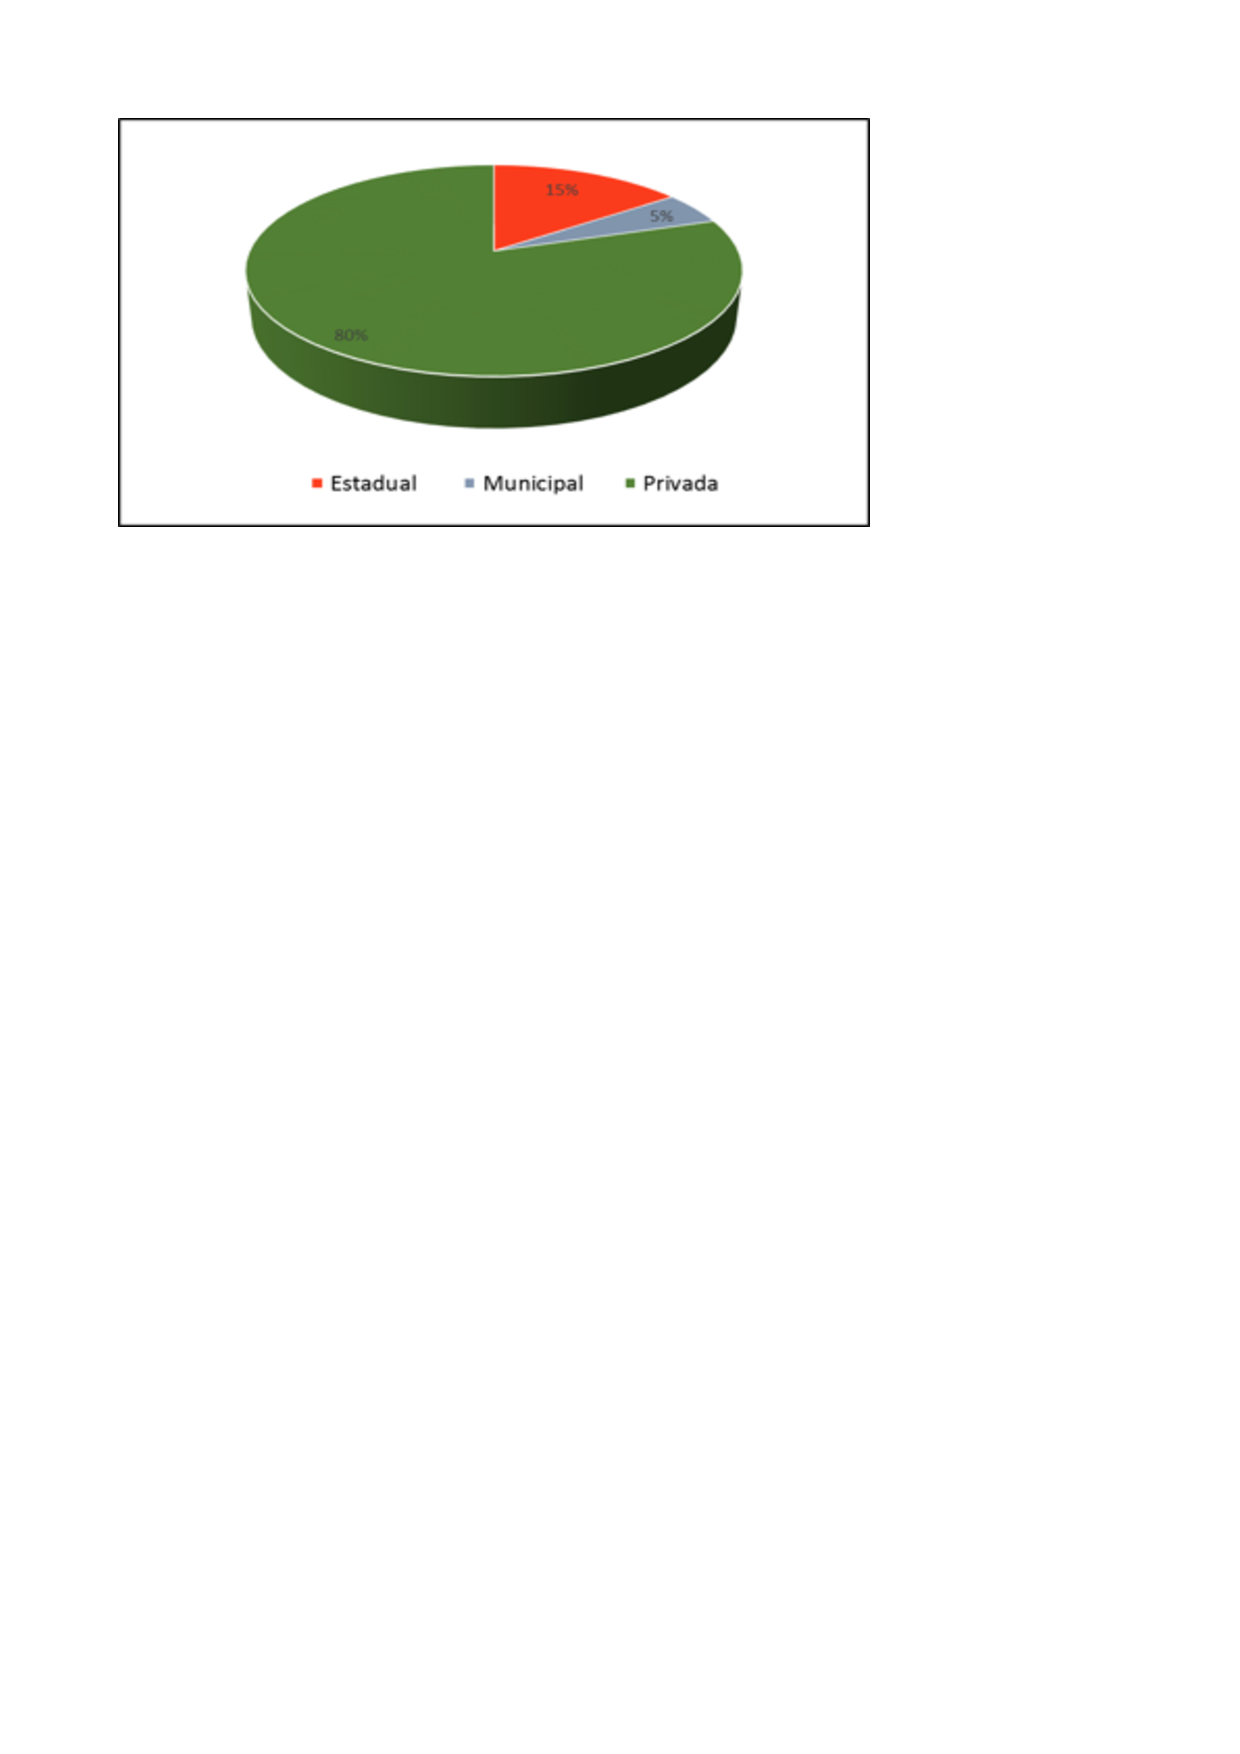
\includegraphics[width=0.8\textwidth]{Grafico1}
\vspace{-0,15cm}
\captionsetup{font=small}
  \caption*{Fonte: Secretaria Municipal de Administra\c{c}\~ao de Horizonte (2009). \citeyear{HOR} \label{Grafico1}}
\end{grafico}


Texto texto texto texto texto texto texto texto texto texto texto texto texto texto texto texto texto texto texto texto texto texto texto texto texto texto texto 
texto texto texto texto texto texto texto texto texto texto texto texto.

Texto texto texto texto texto texto texto texto texto texto texto texto texto texto texto texto texto texto texto texto texto texto texto texto texto texto texto texto texto texto texto texto texto texto texto texto texto texto texto texto texto texto texto texto texto texto.

\vspace{0,5cm}

\begin{grafico}[h]
  \centering
\captionsetup{font=normalsize,skip=0.8pt,width=12.8cm,labelsep=endash}
\caption{Distribui\c{c}\~ao dos documentos analisados por programa de p\'os-gradua\c{c}\~ao}
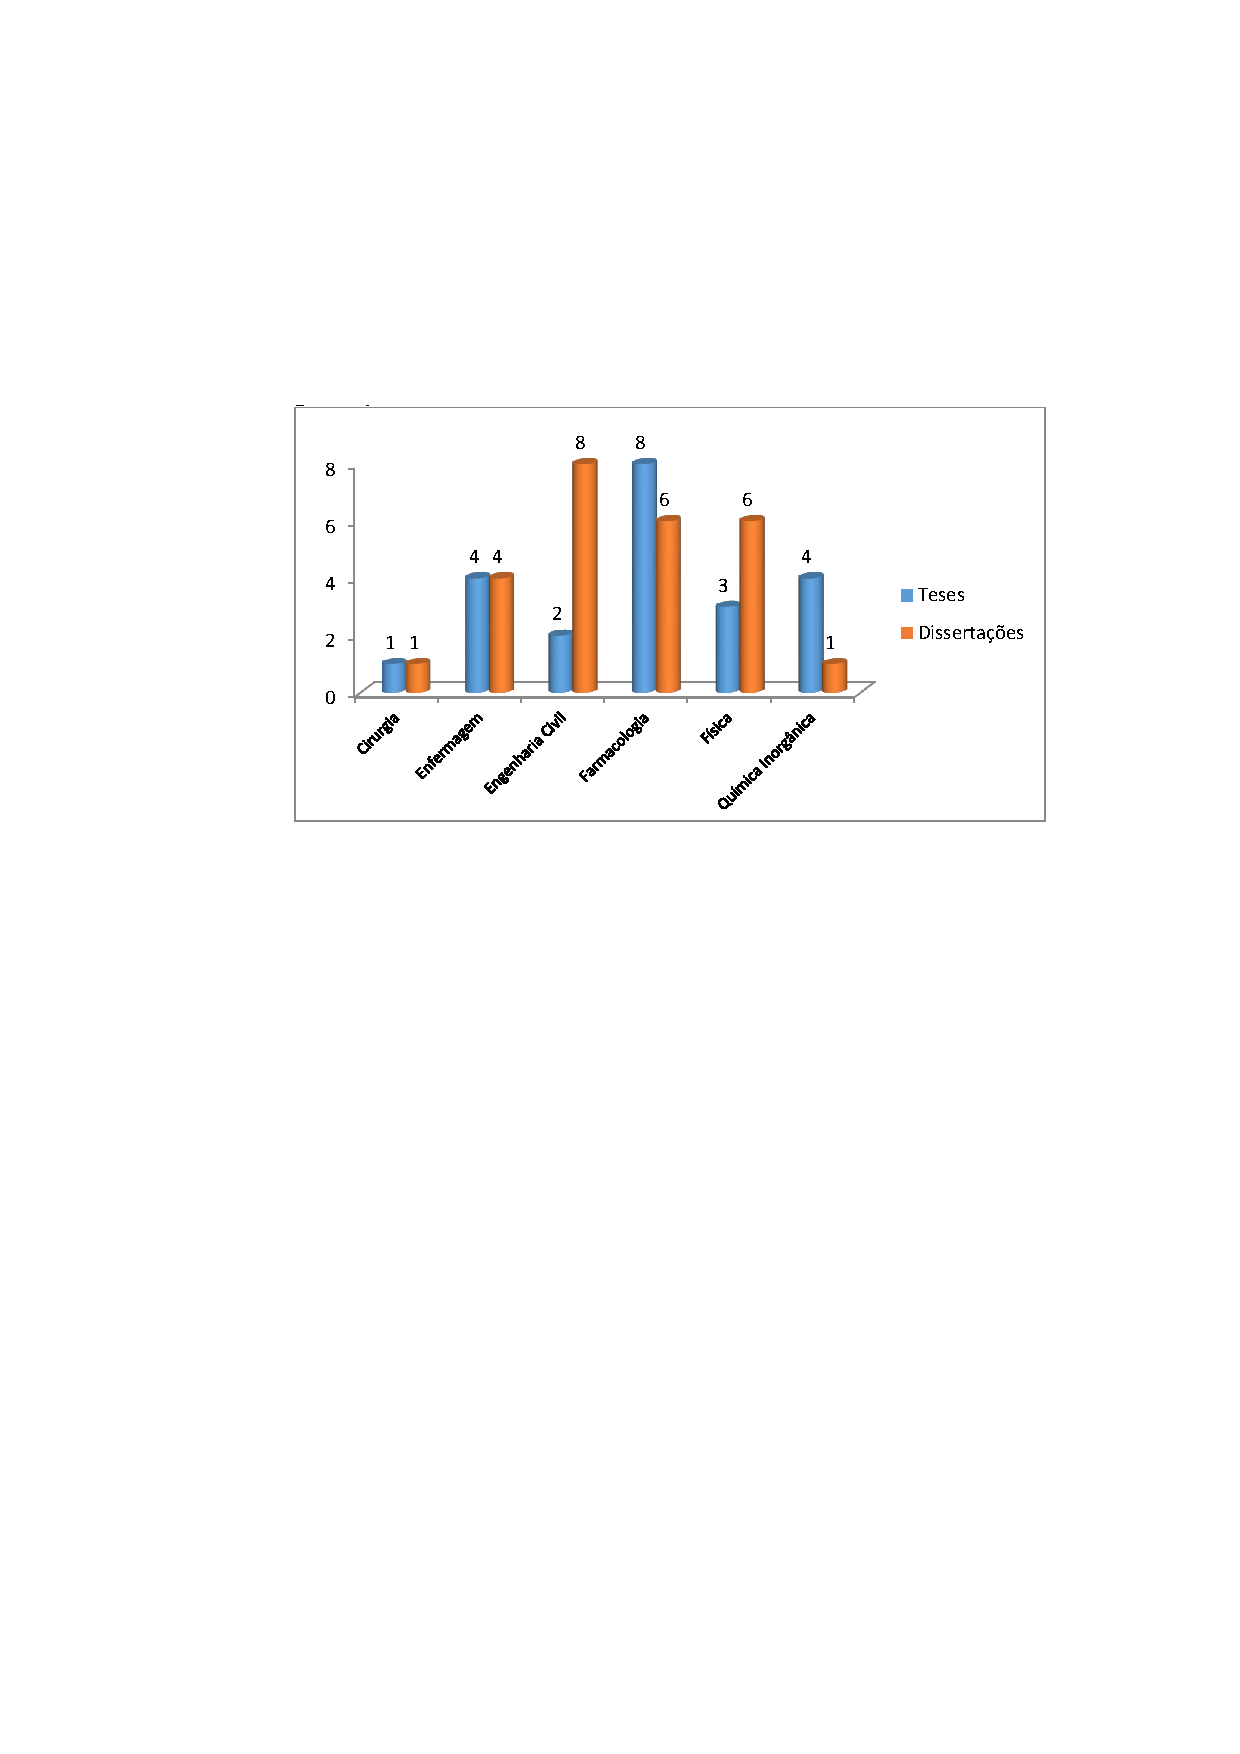
\includegraphics[width=0.8\textwidth]{Grafico2}
\vspace{-0,15cm}
\captionsetup{font=small}
  \caption*{Fonte: Elaborado pelo autor.}
\end{grafico}

Texto texto texto texto texto texto texto texto texto texto texto texto texto texto texto texto texto texto texto texto texto texto texto texto texto texto texto texto texto texto texto texto texto texto texto texto texto texto texto texto texto texto texto texto texto texto.


%%%%%%%%%% -------------------------%%%%%%%%%%%%%%%%%%%%%%%
%%%%%%%%%%  SECAO QUINARIA %%%%%%%%%%%%%%%%%%%%%%%
%%%%%%%%%% --------------------------%%%%%%%%%%%%%%%%%%%%%%%

%Solucao para \subsubsubsection que nao existe no latex
\subparagraph{\rm T\'itulo da se\c c\~ao quin\'aria}

\vspace{0,5cm}

\hspace{2cm}Texto texto texto texto texto texto texto texto texto texto texto texto texto texto texto texto texto texto texto texto texto texto texto texto texto texto texto texto texto texto texto texto texto texto texto texto texto texto texto texto texto texto texto texto texto texto texto texto texto texto texto texto texto texto texto texto texto texto texto texto texto texto.

Texto texto texto texto texto texto texto texto texto texto texto texto texto texto texto texto texto texto texto texto texto texto texto texto texto texto texto texto texto texto texto texto texto texto texto texto texto texto texto texto texto texto texto texto texto texto texto texto texto texto texto texto texto texto texto texto texto texto texto texto texto texto texto texto texto texto texto texto texto texto texto texto texto texto texto texto texto texto texto texto texto texto texto texto texto texto texto texto texto texto texto texto texto texto.

\begin{figure}[h]
  \centering
\captionsetup{width=12.3cm,skip=0pt,labelsep=endash}
\caption{Organiza\c{c}\~ao do conhecimento/Representa\c{c}\~ao da infor-\\ma\c{c}\~ao, Organiza\c{c}\~ao da informa\c{c}\~ao/Representa\c{c}\~ao da informa\c{c}\~ao \label{fig2}}
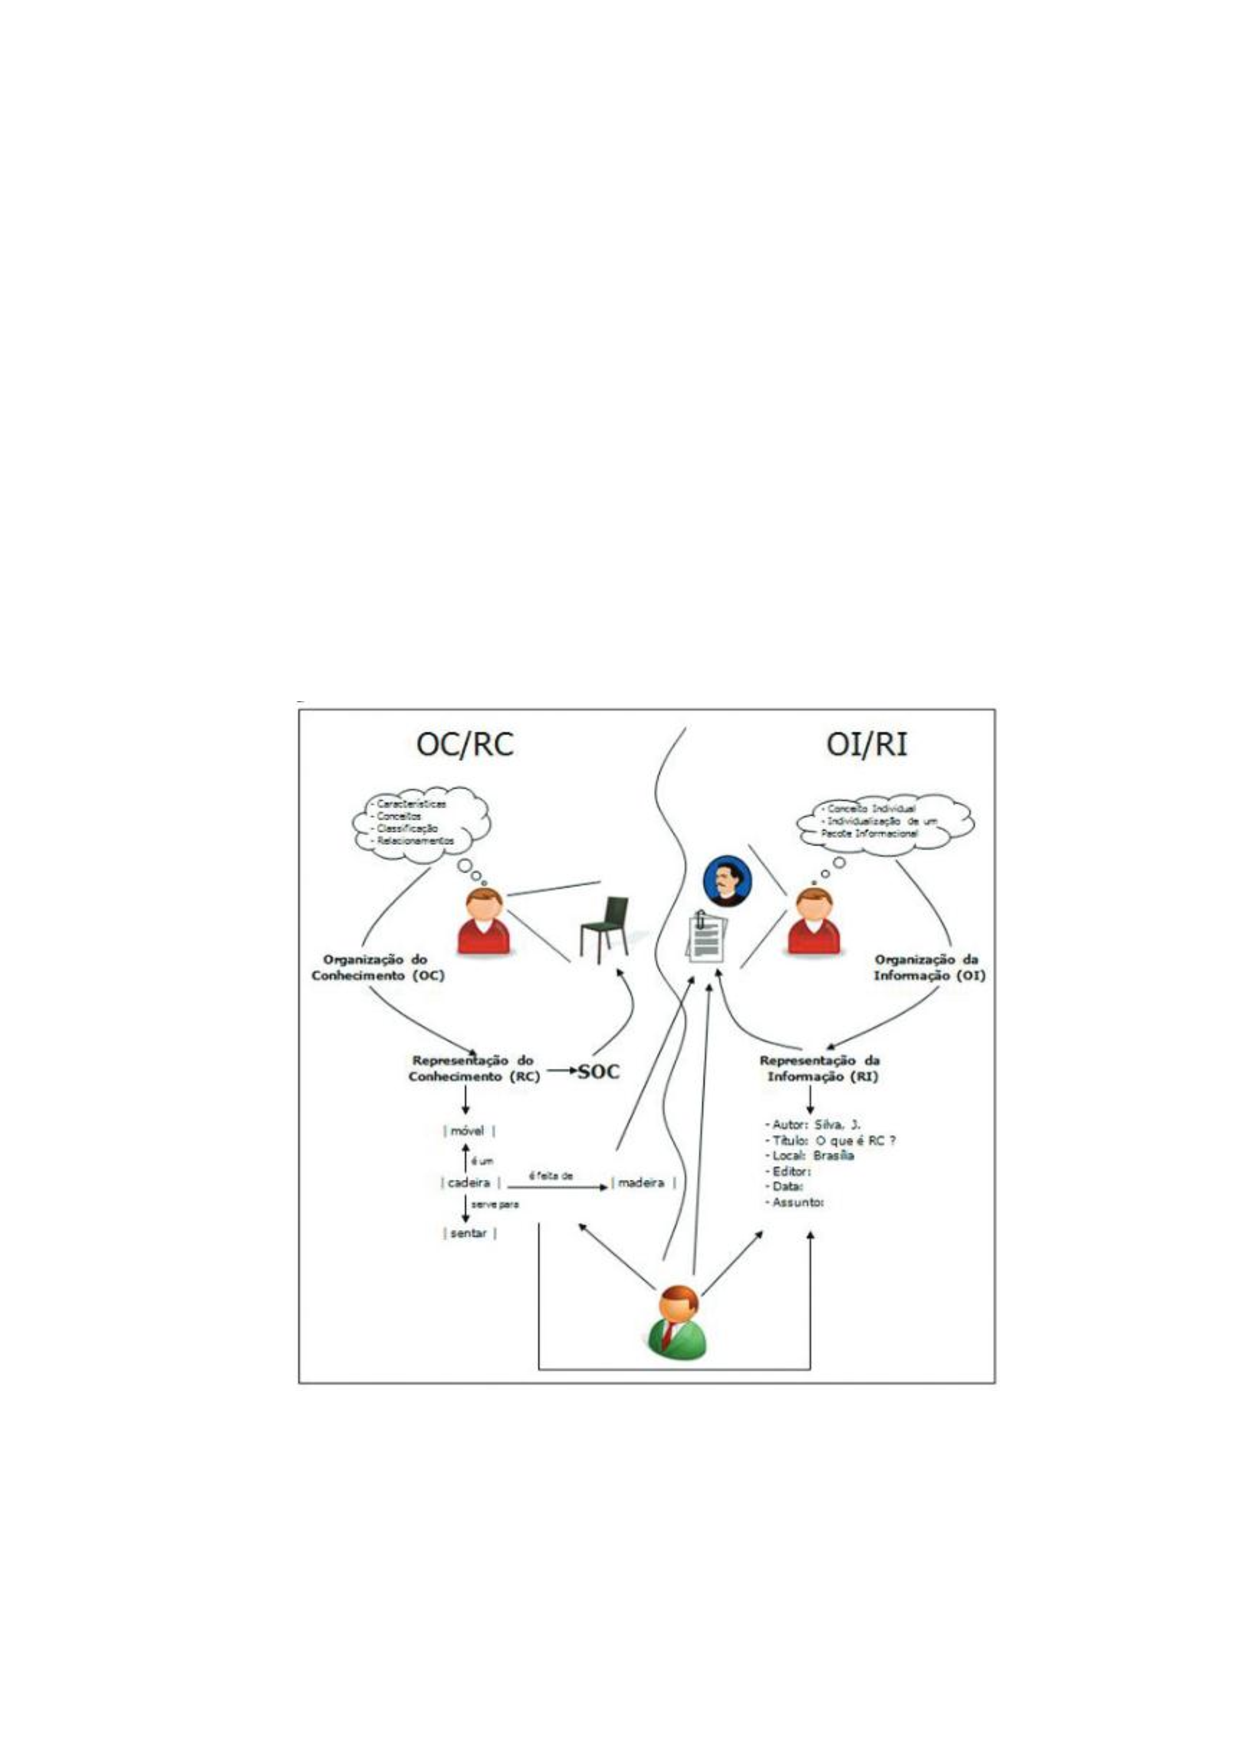
\includegraphics[scale=1.06]{Figura1}
\captionsetup{font=small,position=below,skip=-1pt}
 \caption*{Fonte: Lara e Smit (\citeyear{LaraSmit}).}
\end{figure}


Texto texto texto texto texto texto texto texto texto texto texto texto texto.

\vspace{0,3cm}

\begin{figure}[!h]
  \centering
\captionsetup{font=normalsize,skip=1pt,singlelinecheck=on,labelsep=endash}
\caption{Ciclo da informa\c{c}\~ao}
  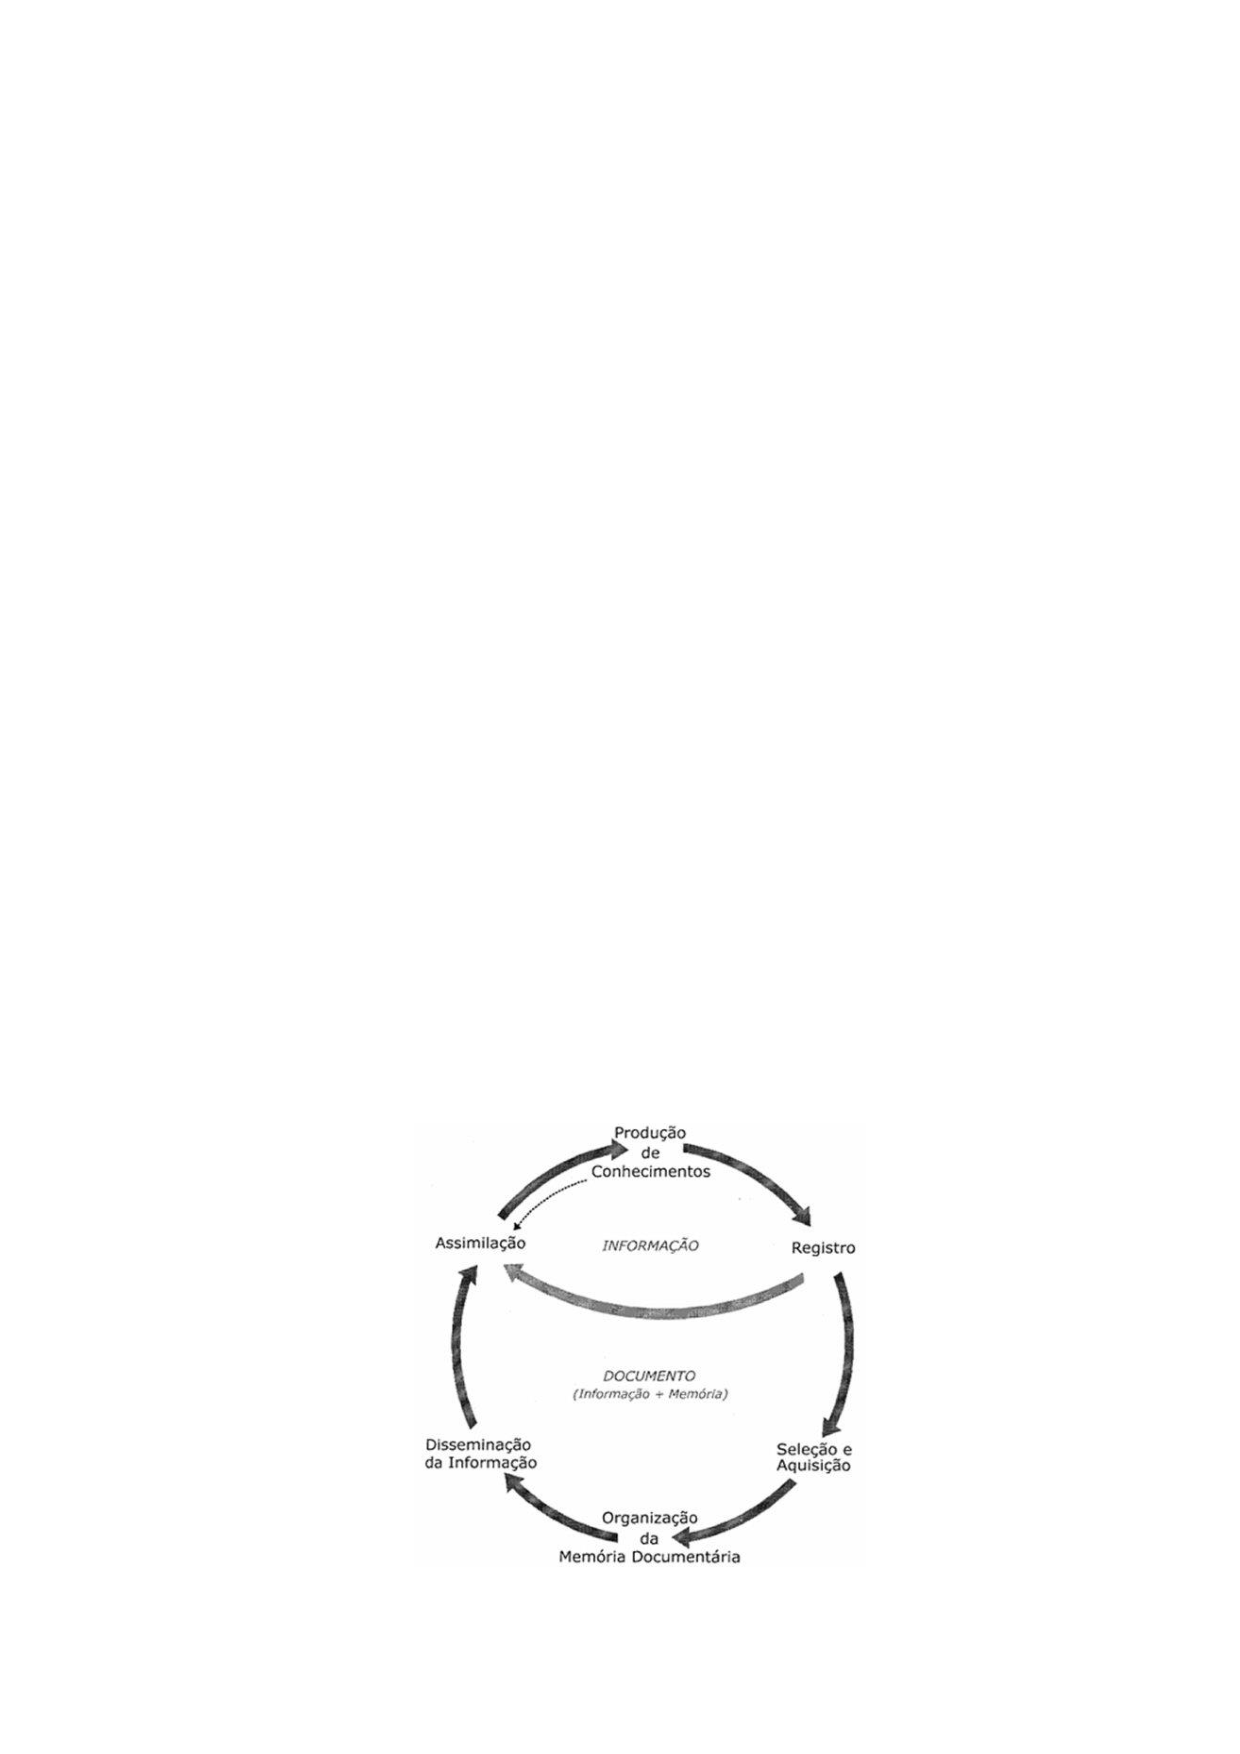
\includegraphics[scale=1]{Figura2}
\captionsetup{font=small,position=below,skip=-1pt}
 \caption*{Fonte: Trist\~ao, Fachin e Alarcon (\citeyear{Trist}).}
\end{figure}


Texto texto texto texto texto texto texto texto texto texto texto texto texto texto texto texto texto texto texto texto texto texto texto texto texto texto texto texto texto texto texto texto texto texto texto texto texto texto texto texto texto texto texto texto texto texto texto texto texto texto texto texto texto texto texto texto texto texto texto texto texto texto texto texto texto texto texto texto texto texto texto texto texto texto texto texto texto texto texto texto texto texto texto texto texto texto texto texto texto.

Texto texto texto texto texto texto texto texto texto texto texto texto texto texto texto texto texto texto texto texto texto texto texto texto texto texto texto texto texto texto texto texto texto texto texto texto texto texto texto texto texto texto texto texto texto.

\pagebreak  %quebra de pagina
\newpage

%%%%%%%%%% ----------------------------------------%%%%%%%%%%%%%%%%%%%%%%%
%%%%%%%%%%  TERCEIRA SECAO PRIMARIA %%%%%%%%%%%%%%%%%%%%%%%
%%%%%%%%%% ----------------------------------------%%%%%%%%%%%%%%%%%%%%%%%

\pagestyle{myheadings}

\onehalfspacing

\section{\normalsize{T\'ITULO DA SE\c C\~AO PRIM\'ARIA}}

\vspace{0,2cm}

\hspace{2cm} Texto texto texto texto texto texto texto texto texto texto texto texto texto texto texto texto texto texto texto texto texto texto texto texto texto texto texto texto texto texto texto texto texto texto texto texto texto texto texto texto texto texto texto texto texto texto, conforme Tabela \ref{tab1}.

\vspace{0,3cm}

\begin{table}[h]
  \centering
\captionsetup{margin={9pt,14pt},font=normalsize,skip=0.5pt,labelsep=endash}
\caption{Distribui\c c\~ao dos documentos analisados por programa de p\'os-gradua\c c\~ao\label{tab1}}
        \begin{tabular}{l|c|c|c}
           \specialrule{1pt}{0pt}{0pt}
    \multirow{2}{*}{\textbf{Programas de p\'os-gradua\c{c}\~ao~~~~~~~}}     
    & \multicolumn{2}{c|}{\textbf{Categoria}}  &  \multirow{2}{*}{\textbf{~Total~}} \\
            \cline{2-3}
             & \textbf{~~~~~Teses~~~~~} & \textbf{Disserta\c{c}\~oes} &  \\
            \hline
            Cirurgia  & 1 & 1 & 2 \\
            Enfermagem & 4 &4 & 8 \\
            Engenharia Civil & 2 & 8 & 10 \\
            Farmacologia & 8 & 6 & 14 \\
            F\'isica & 3 & 6 & 9 \\
            Qu\'imica Inorg\^anica & 4 &1 & 5 \\
            {\bf Total}   & {\bf 22} & {\bf 26} & {\bf 48} \vspace{-0.6mm}\\ \bottomrule[1pt]        
        \end{tabular}
\captionsetup{margin={10pt,10pt},font=small,skip=0pt,position=below}
\caption*{Fonte: Elaborada pelo autor.}
\end{table}

Texto texto texto texto texto texto texto texto texto texto texto texto texto texto texto texto texto texto texto texto texto texto 
texto texto texto texto texto texto texto texto texto texto texto texto texto texto texto texto texto texto texto texto texto texto 
texto texto texto texto texto.

Texto texto texto texto texto texto texto texto texto texto texto texto texto texto texto texto texto texto texto texto texto texto 
texto texto texto texto texto texto texto texto texto texto texto texto texto texto (Tabela 2).

\vspace{0,5cm}

\begin{table}[h]
  \centering
\captionsetup{margin={23pt,22pt},font=normalsize,skip=0.5pt,labelsep=endash}
\caption{Popula\c{c}\~ao brasileira por situa\c c\~ao em domic\'ilio em 2003 \label{tab2}}
\begin{tabular}{lccc}
 \specialrule{1pt}{0pt}{0pt}
{\bf Situa\c c\~ao do Domic\'ilio}~~~  \vline &  {\bf ~Mulheres~~~} \vline & {\bf ~Homens~~~} \vline & {\bf Total} \\
\hline
Urbana & 41.115.439 & 79,972492 & 79.972.370  \\
Rural             & 18.479.893 & 19.507.477 & 37.982.370  \\
{\bf Total}      & {\bf 59.595.332} & {\bf 58.364.969} & {\bf 117.960.301} \\
 \specialrule{1pt}{0pt}{0pt}
\end{tabular}
\captionsetup{margin={24pt,20pt},font=small,position=below,skip=0pt}
 \caption*{Fonte: \cite{INST} (2003).}
\end{table}


Texto texto texto texto texto texto texto texto texto texto texto texto texto texto texto texto texto texto 
texto texto texto texto texto texto texto texto texto texto texto texto texto texto texto texto texto texto 
texto texto texto texto texto texto texto texto texto texto texto texto texto texto texto texto texto texto 
texto texto texto texto texto texto texto.

\pagebreak  %quebra de pagina


%%%%%%%%%% -------------------%%%%%%%%%%%%%%%%%%%%%%%
%%%%%%%%%%  CONCLUSAO %%%%%%%%%%%%%%%%%%%%%%%
%%%%%%%%%% -------------------%%%%%%%%%%%%%%%%%%%%%%%

\pagestyle{myheadings}

\onehalfspacing

\section{\normalsize{CONCLUS\~AO}}

\vspace{0,2cm}

\hspace{2cm} Parte final do texto na qual se apresentam as conclus\~oes apoiadas no desenvolvimento do assunto. 
\'E a recapitula\c c\~ao sint\'etica dos resultados obtidos. Pode apresentar recomenda\c c\~oes e sugest\~oes para pesquisas futuras.

Texto texto texto texto texto texto texto texto texto texto texto texto texto texto texto texto texto texto texto texto texto texto texto texto texto 
texto texto texto texto texto texto texto texto texto texto texto texto texto texto texto texto texto texto texto texto texto texto texto texto texto 
texto texto texto texto texto texto texto texto texto texto texto texto texto texto texto texto texto texto texto texto texto texto texto texto texto texto texto.

Texto texto texto texto texto texto texto texto texto texto texto texto texto texto texto texto texto texto texto texto texto texto texto texto texto texto 
texto texto texto texto texto texto texto texto texto texto texto texto texto texto texto texto texto texto texto texto texto texto texto texto texto texto t
exto texto texto texto texto texto texto texto texto.

Texto texto texto texto texto texto texto texto texto texto texto texto texto texto texto texto texto texto texto texto texto texto texto texto texto texto 
texto texto texto texto texto texto texto texto texto texto texto texto texto texto texto texto texto texto texto texto texto texto texto texto texto texto 
texto texto texto texto texto texto texto texto texto texto texto texto texto texto texto texto texto texto texto texto texto texto texto texto texto.

Texto texto texto texto texto texto texto texto texto texto texto texto texto texto texto texto texto texto texto texto texto texto texto texto texto texto 
texto texto texto texto texto texto texto texto texto texto texto texto texto texto texto texto texto texto texto texto texto texto texto texto texto texto 
texto texto texto texto texto texto texto texto texto texto texto texto texto texto texto texto texto texto texto texto texto texto texto texto texto. 

\pagebreak  %quebra de pagina

%%%%%%%%%% ---------------------%%%%%%%%%%%%%%%%%%%%%%%
%%%%%%%%%%  REFERENCIAS %%%%%%%%%%%%%%%%%%%%%%%
%%%%%%%%%% ---------------------%%%%%%%%%%%%%%%%%%%%%%%


\renewcommand\refname{\centerline {\normalsize REFER\^ENCIAS}}
\addcontentsline{toc}{section}{\protect\numberline{}{\bf REFER\^ENCIAS}}

\thispagestyle{myheadings}

\pagebreak  %quebra de pagina

\newpage

%%%%%%%%%% ---------------------%%%%%%%%%%%%%%%%%%%%%%%
%%%%%%%%%%  REFERENCIAS %%%%%%%%%%%%%%%%%%%%%%%
%%%%%%%%%% ---------------------%%%%%%%%%%%%%%%%%%%%%%%

\bibliographystyle{ufctex}

\setlength\parskip{1cm}       %comando para espacamente do nome REFERENCIA
\setlength{\bibhang}{0em}  %comando para nao identar segunda linha
\singlespacing                       %comando para espacamento
\setlength{\bibsep}{1,5em}  %espaçamentos entre referencias
\flushleft %Justificar a esquerda as referencias
\bibliography{Template}

\newpage
\end{document}